% !TEX root = ../main.tex

% 3 p. 92
[\SI{80}{\percent} (b)] Een pijl wordt verticaal van de grond omhooggeschoten en bereikt na \SI{2,8}{s} het hoogste punt. Bepaal deze hoogte.
\begin{oplossing}
\item[Gegeven]\SI{2,8}{s}
\item[Gevraagd]$v_0$, $x_{max}$

\item[Oplossing]\begin{minipage}[t]{0.6\linewidth}
	Op het hoogste punt is de snelheid van de pijl nul. Aangezien we weten hoe lang hij onderweg is en de pijl per seconde \SI{9,81}{m/s^2} trager omhoog vliegt, kunnen we hieruit de beginsnelheid bepalen. 
	
	We kiezen de referentie-as met de oorsprong op de grond. De versnellingscomponent is dan het tegengestelde van de valversnelling, $a=-g$.
\end{minipage}%
\begin{minipage}[t]{0.37\linewidth}
	\raisebox{1ex-\height}{%
	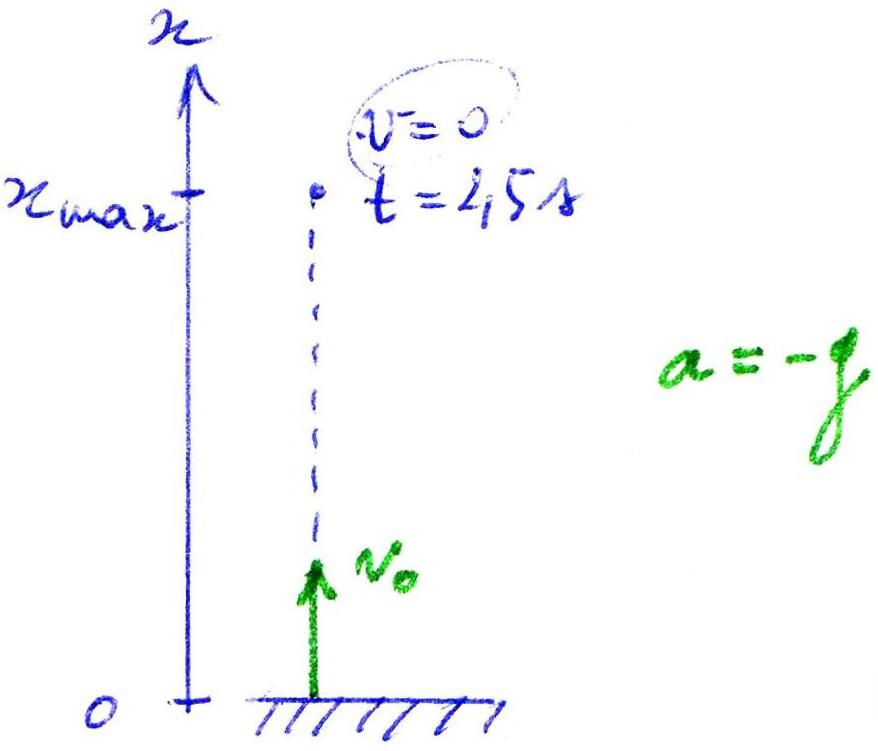
\includegraphics[height=5cm]{55p44}%
	}
\end{minipage}

We krijgen:
\begin{equation*}
v=0\Leftrightarrow v_0-gt=0\Leftrightarrow v_0=gt
\end{equation*}
Dat is in grootte gelijk aan \SI{27}{m/s}.\footnote{Als je voor de valversnelling $g=\SI{10}{m/s^2}$ gebruikt, is de beginsnelheid gelijk aan \SI{28}{m/s}} Nu dat we ook de beginsnelheid kennen, vinden we de afgelegde afstand, wat ook de maximale hoogte is:
\begin{equation*}
x=v_0t-\frac{1}{2}gt^2=(gt)t-\frac{1}{2}gt^2=\frac{1}{2}gt^2
\end{equation*}
Vullen we de getalwaardes in, dan vinden we \SI{38}{m}
\newline
\newline
Merk op dat deze afstand gelijk is aan de afstand die de pijl vanuit rust zou afleggen bij een vrije val die \SI{2,8}{s} duurt. Dat is niet heel verwonderlijk; de vertraging naar boven toe is namelijk gelijk aan de versnelling bij het vallen naar beneden. Wiskundig loopt de symmetrieas van een parabool door de top. 

\end{oplossing}